\documentclass{article}
\usepackage[utf8]{inputenc}
\usepackage[margin=1in]{geometry}
\usepackage[shortlabels]{enumitem}
\usepackage[export]{adjustbox}
\usepackage{amsfonts}
\usepackage{amsmath}
\usepackage{amssymb}
\usepackage{array}
\usepackage{etoolbox}
\usepackage{mathrsfs}
\usepackage{listings}
\usepackage{graphicx}
\let\n\newline
\let\t\text


\newcommand\ol[1]{\ensuremath{\overline{#1}}} % doesnt show up in preview :(
\newcolumntype{L}{>$l<$}

\title{Knowledge Base}
\author{Jonathan Yu}	

\preto\array{\setcounter{magicrownumbers}{0}}
\newcounter{magicrownumbers}
\newcommand\rownumber{\stepcounter{magicrownumbers}\arabic{magicrownumbers}}

\begin{document}
\renewcommand{\arraystretch}{1.5}
\maketitle
\begin{enumerate}
	\item \textbf{The president walked around during his speech, asking important questions that didn't always have answers.}
	\item In my PSG tree, I found the following phrase terms:
		\begin{itemize}
			\item S - This is a declarative clause
			\item NP - This is a noun phrase
			\item VP - This is a verb phrase
			\item ADVP - This is an adverp phrase
			\item PP - This is a prepositional phrase
			\item SBAR - This is a clause introduced by a subordinating conjunction
		\end{itemize}
		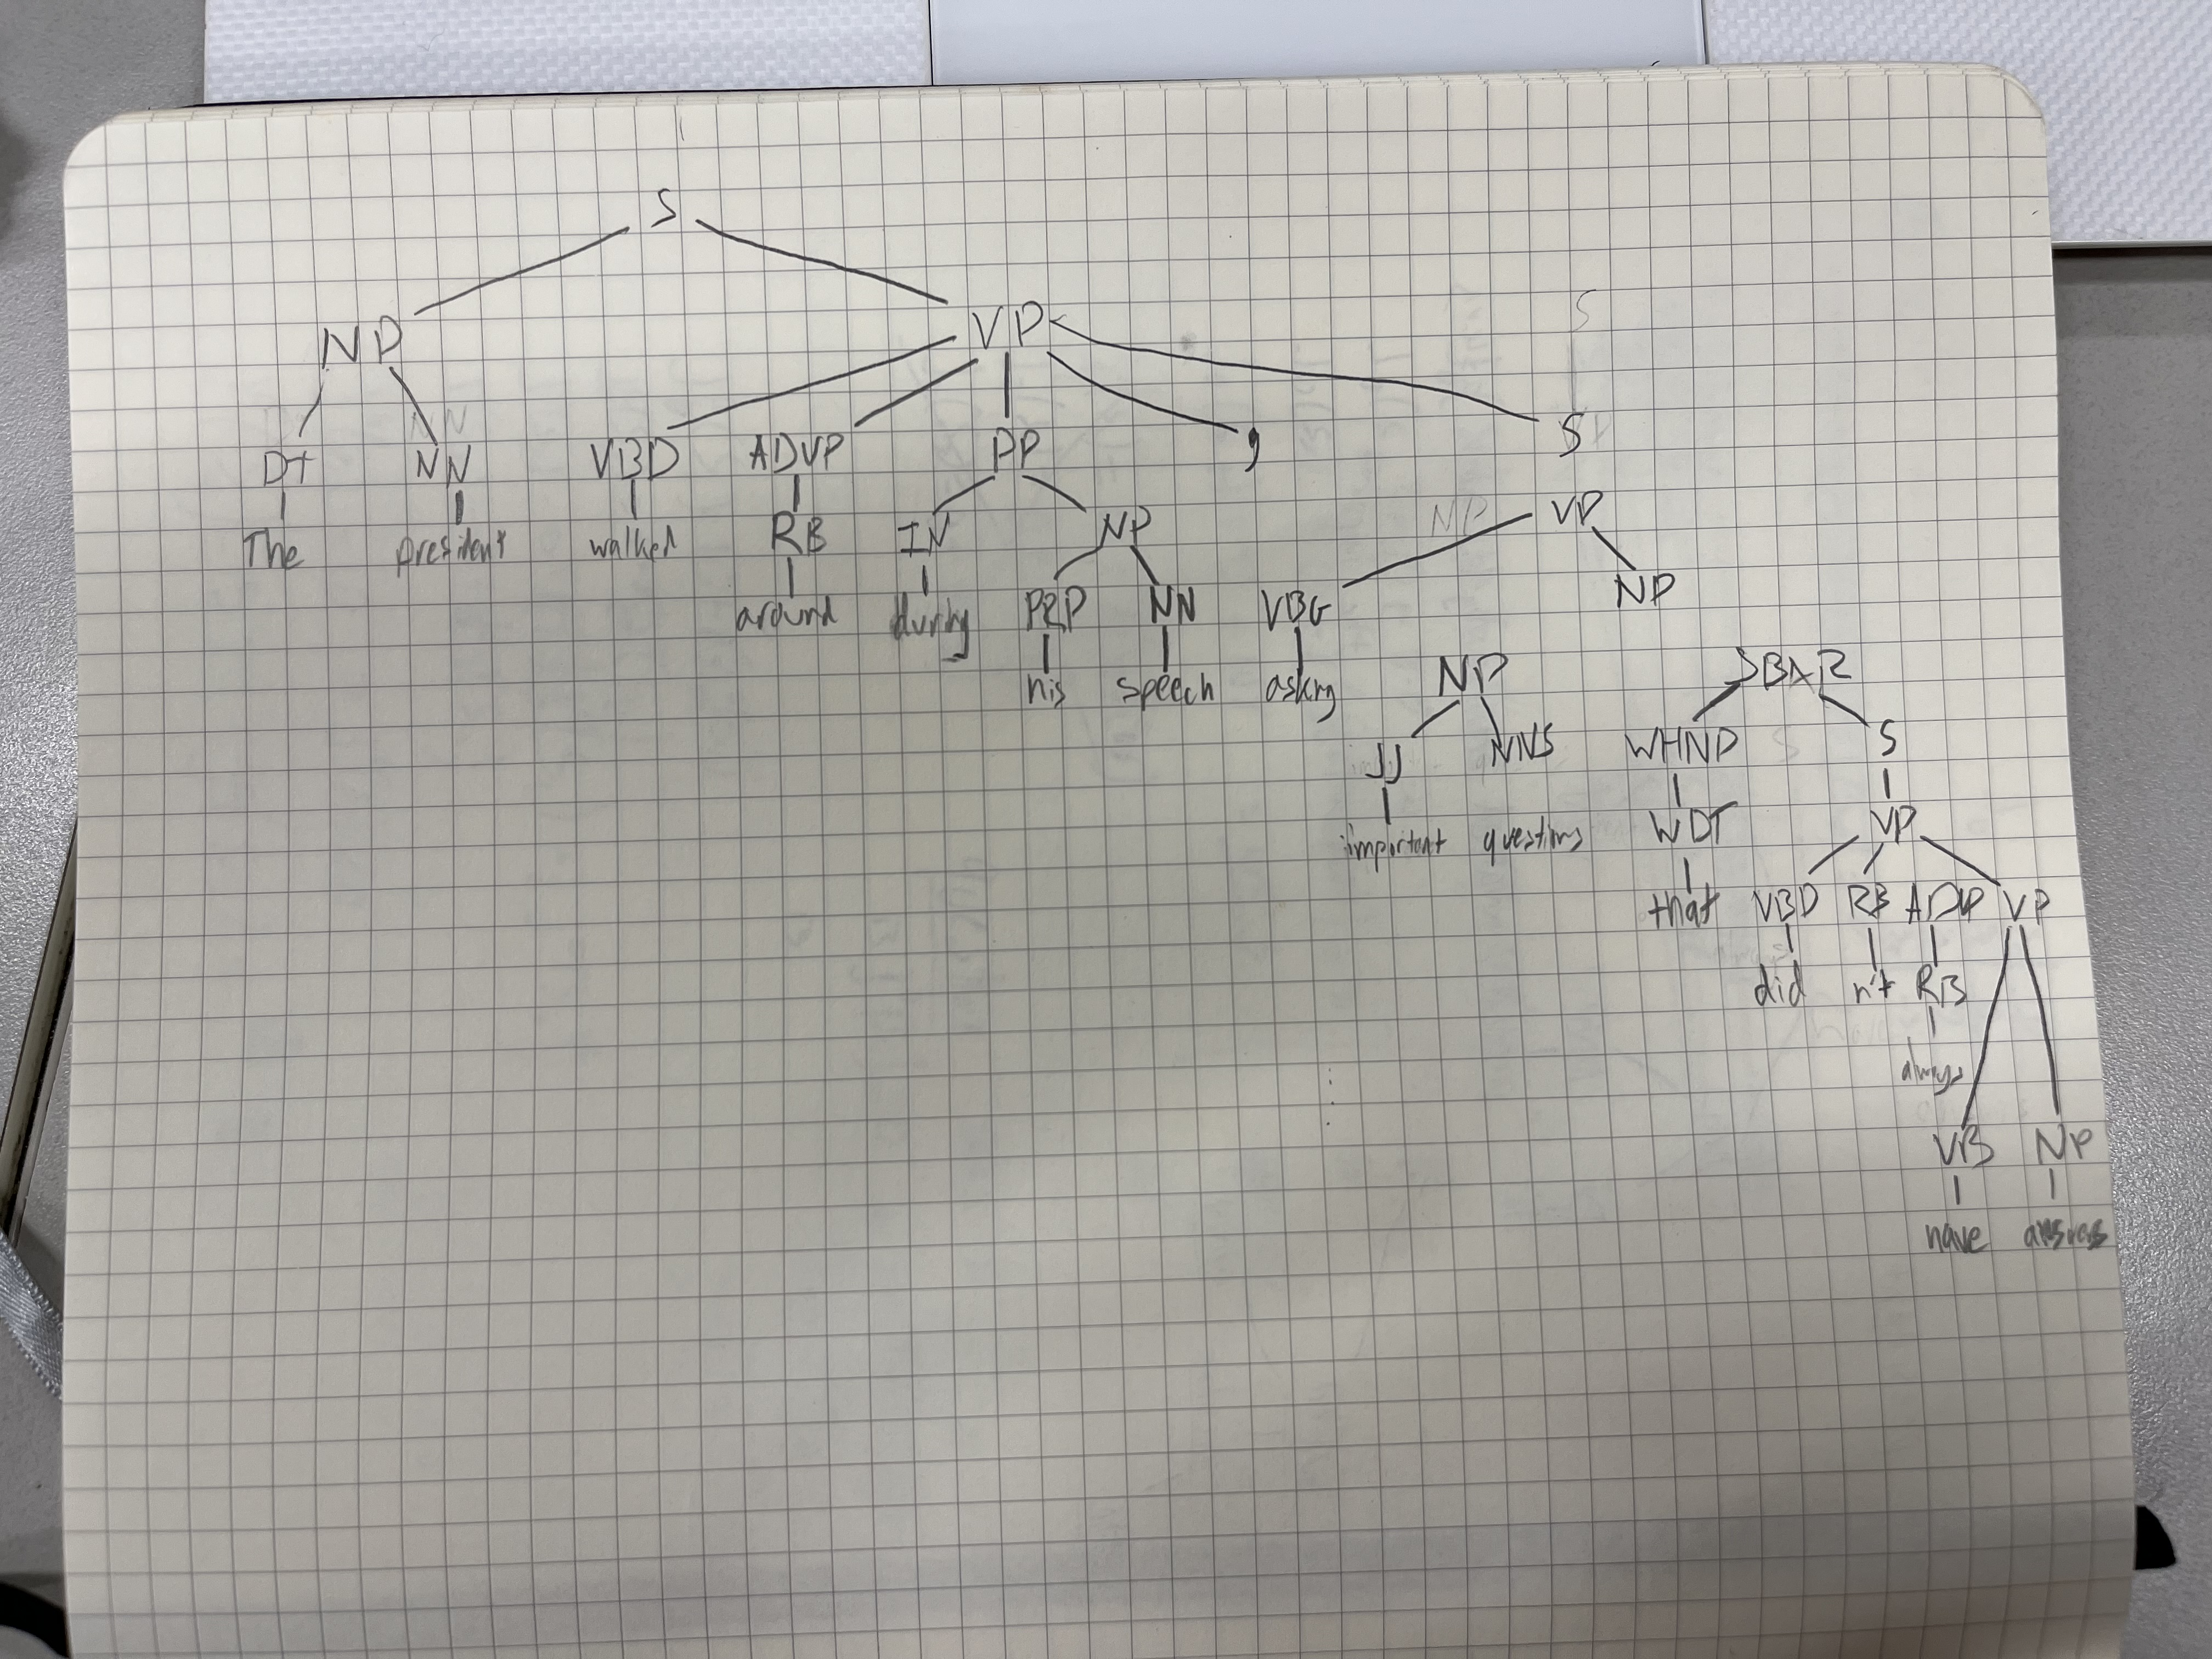
\includegraphics[width=12cm]{IMG-1534.jpg}
	\item In my dependency parse, I found the following dependency terms:
		\begin{itemize}
			\item nsubj - nominal subject. This is a noun phrase which is the subject of a clause
			\item det - determiner. This is the relation in a noun phrase between the noun and its determiner
			\item advmod - adverb modifier. This is a non-clausal adverb that modifies a word
			\item prep - prepositional modifier. This is a prepositional phrase that modifies the meaning of a word
			\item pobj - object of a preposition. This is the head of a noun phrase following the preposition
			\item amod - adjectival modifier. An adjectival phrase that modifies the meaning of a noun phraseo
			\item ccomp - clausal component. A dependent clause with an internal subject which functions like an object of the verb or adjective
			\item neg - negation modifier. Relation between the negation word and the word it modifies
			\item mark - marker. The word indroducing a finite clause subordinate to another clause
			\item aux - auxiliary. A non-main verb of a clause
		\end{itemize}
		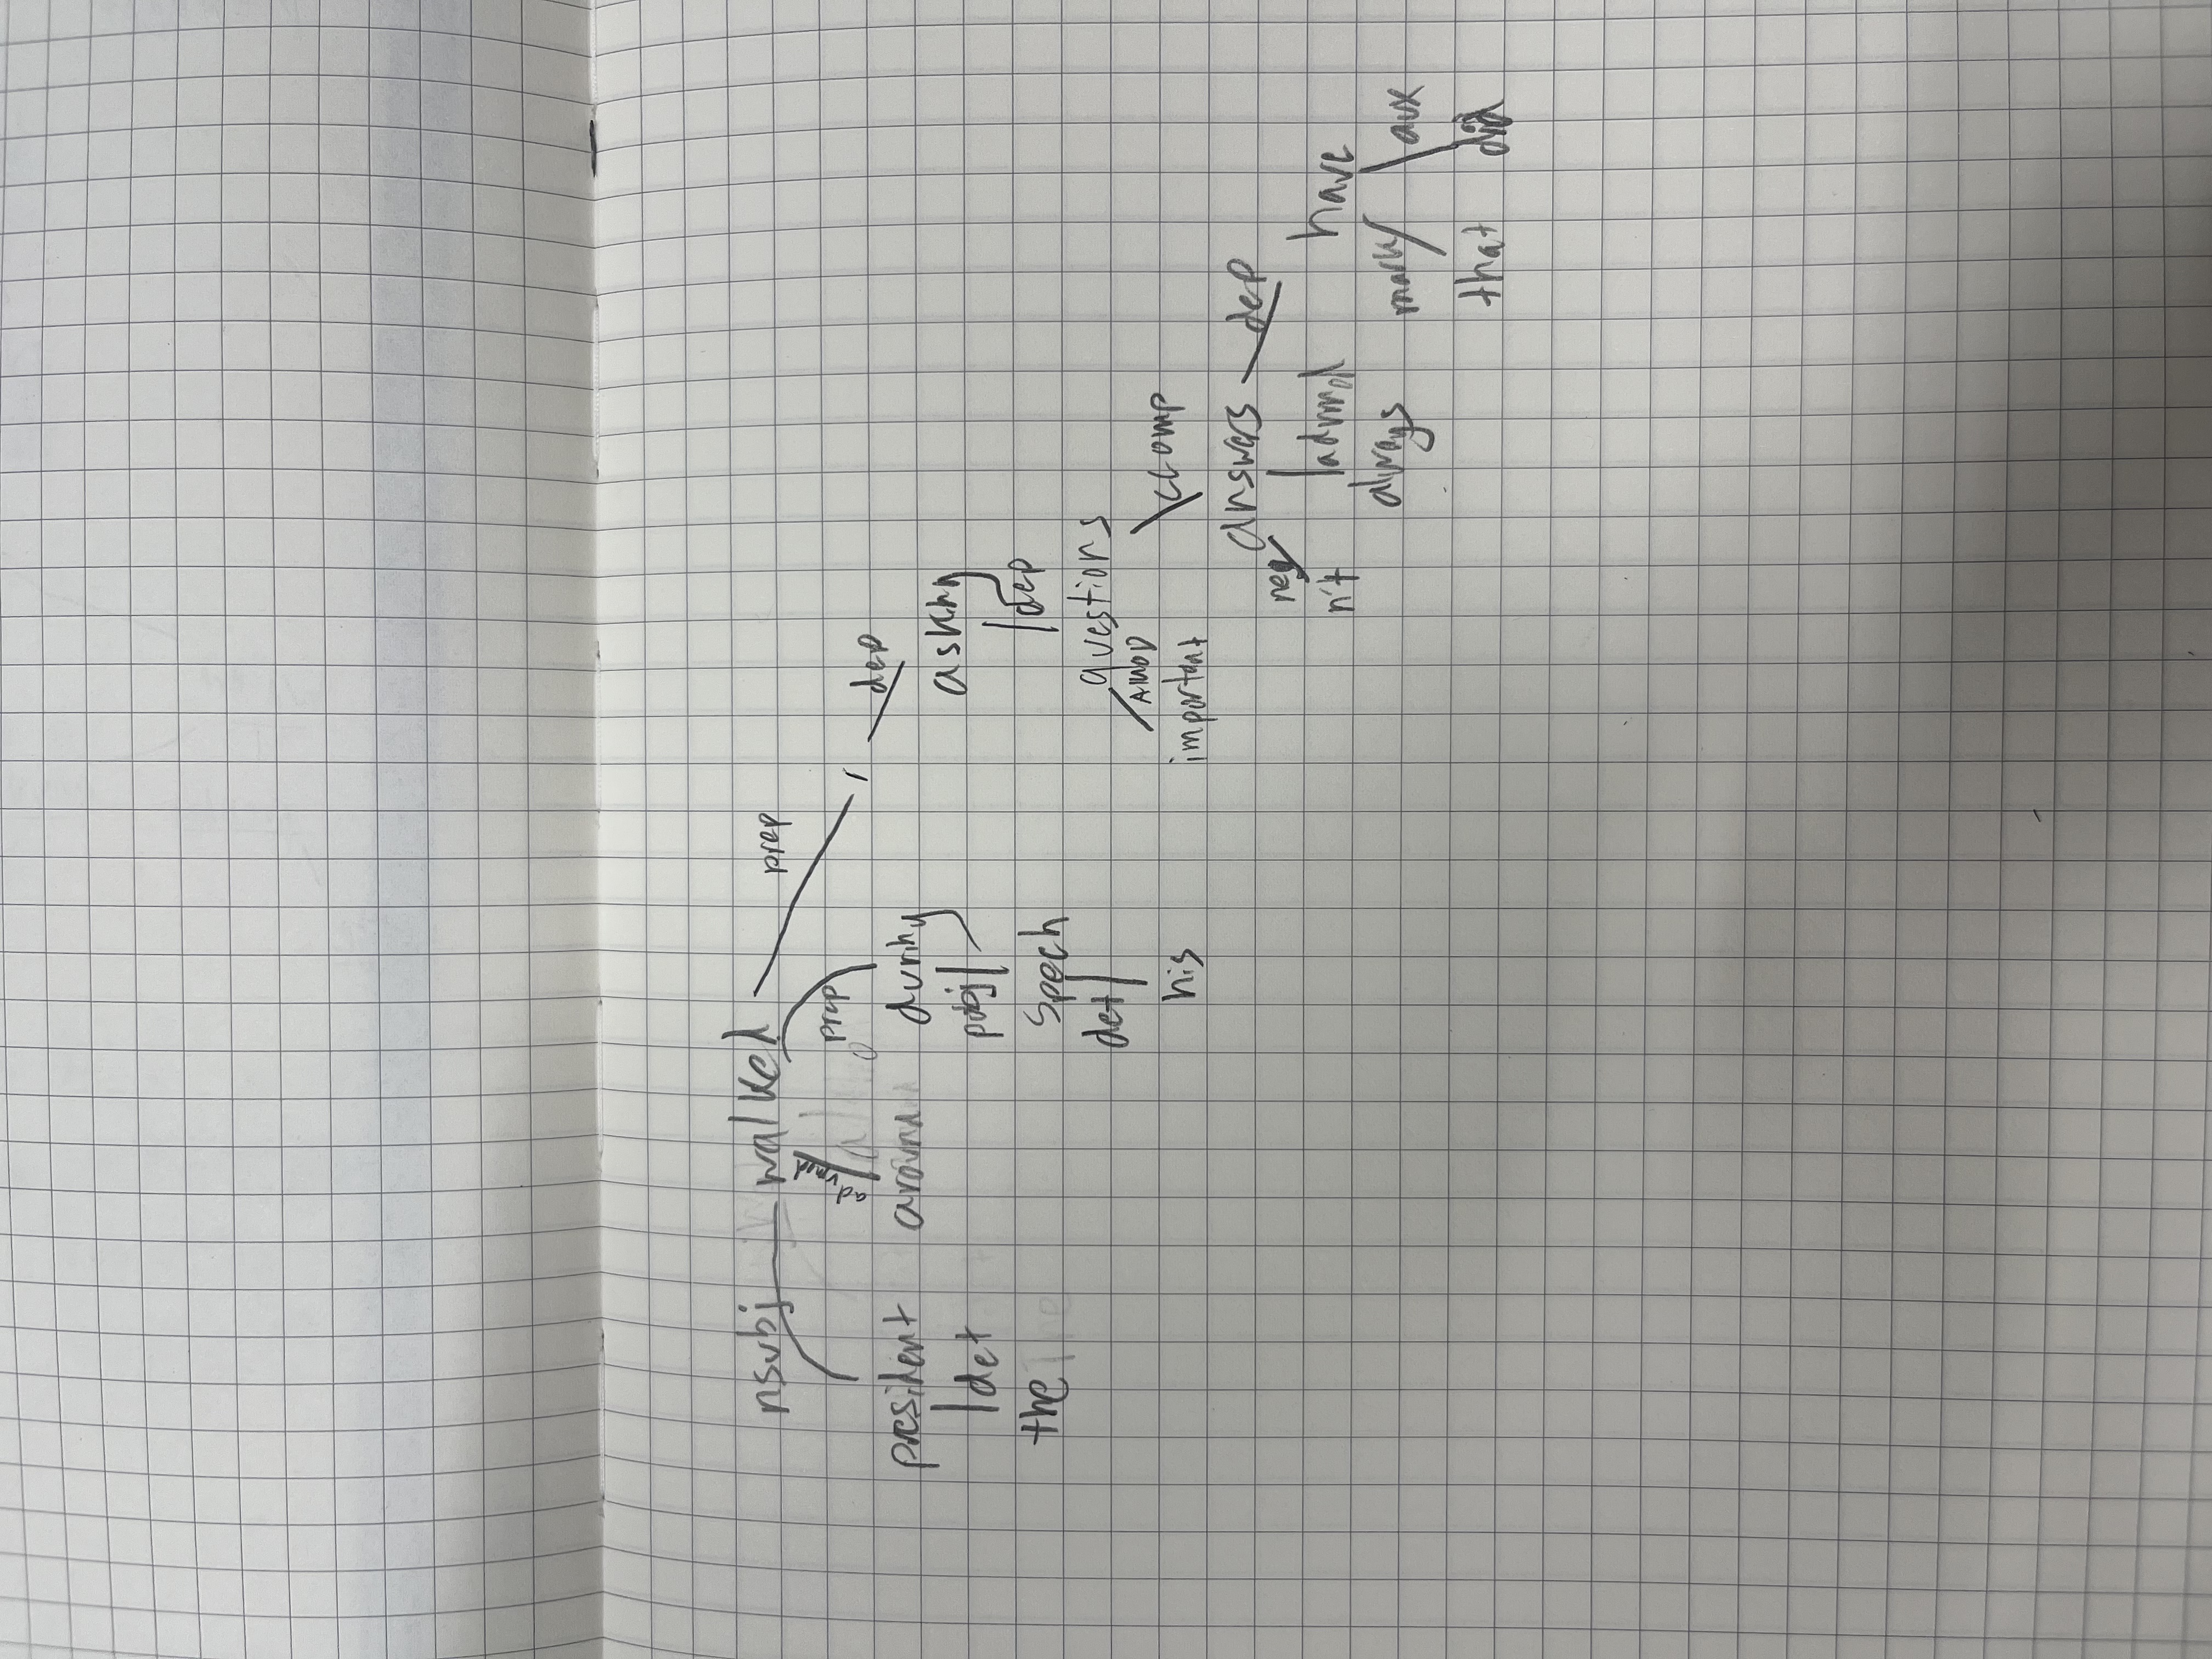
\includegraphics[width=12cm]{IMG-1535.jpg}

	\item I will define all modifiers here: \begin{itemize}
		\item DIR - indicates motion along a path (a direction)
		\item TMP - indicates when an action happend
		\item ADV - miscillaenous modifier
		\item NEG - indicates the action is negated
		\end{itemize}
		The following is the SRL parse for my sentence.
		\begin{itemize}
			\item Predicate 1: walked\n
				The president is ARG0 since he's the one performing the verb, walked.
			\begin{itemize}
				\item ARG0: The president
				\item V: walked
				\item ARGM-DIR: around
				\item ARGM-TMP: during his speech
				\item ARGM-ADV: asking important questions that did n't always have answers
			\end{itemize}

			\item Predicate 2: asking\n
				The presidnet is still ARG0 since he's the one performing the asking. The imporant questions clause is ARGM1L because this is the subject of the verb asking.
				\begin{itemize}
				\item ARG0: The president
				\item V: asking
				\item ARGM1L important questions that did n't always have answers
			\end{itemize}

			\item Predicate 3: did \n
				This predicate has no arguments becuase it actually isn't important with regards to the meaning of the sentence, the only thing that's important is the negation attached to it.
			\begin{itemize}
				\item V: did
			\end{itemize}

			\item Predicate 4: have \n
				The ARG0 for this predicate is important questions, which is then modified by R-ARG0 "that". Then, we can see that the ARG1 is what the questions don't have: answers.
			\begin{itemize}
				\item ARG0: important questions
				\item R-ARG0: that
				\item ARGM-NEG: n't
				\item ARGM-TMP: always
				\item V: have
				\item ARG1: answers
			\end{itemize}
		\end{itemize}

	\item In my opinion, I think that PSG trees are very strong at determining proper grammatical relationships. The issue, however is that they aren't as good at extracting meaning as dependency parsing. I think dependency parsing is the most powerful in terms of extracting meaning because it shows direct relations between the words. This helps figure out semantic meaning of the sentence. SRL parse come close in terms of robustness when parsing the meaning of sentences, however It's more complex than a dependency parse. From all of this, my favorite parse is the dependency parse.


\end{enumerate}


\end{document}	